% 
% Annual Cognitive Science Conference
% Sample LaTeX Paper -- Proceedings Format
% 

% Original : Ashwin Ram (ashwin@cc.gatech.edu)       04/01/1994
% Modified : Johanna Moore (jmoore@cs.pitt.edu)      03/17/1995
% Modified : David Noelle (noelle@ucsd.edu)          03/15/1996
% Modified : Pat Langley (langley@cs.stanford.edu)   01/26/1997
% Latex2e corrections by Ramin Charles Nakisa        01/28/1997 
% Modified : Tina Eliassi-Rad (eliassi@cs.wisc.edu)  01/31/1998
% Modified : Trisha Yannuzzi (trisha@ircs.upenn.edu) 12/28/1999 (in process)
% Modified : Mary Ellen Foster (M.E.Foster@ed.ac.uk) 12/11/2000
% Modified : Ken Forbus                              01/23/2004
% Modified : Eli M. Silk (esilk@pitt.edu)            05/24/2005
% Modified: Niels Taatgen (taatgen@cmu.edu) 10/24/2006

%% Change ``a4paper'' in the following line to ``letterpaper'' if you are
%% producing a letter-format document.

\documentclass{article} % For LaTeX2e

\usepackage{nips12submit_e,times}
\usepackage{pslatex}
\usepackage{amsmath}
\usepackage{amsfonts}
\usepackage{latexsym}
\usepackage{amssymb}
\usepackage{apacite}
\usepackage{graphicx}
\usepackage{xspace}
\usepackage{multirow}
\usepackage{array}
\usepackage{caption}
\usepackage{subcaption}

\newcommand{\dictionary}{\ensuremath{\mathcal{D}}\xspace}
\newcommand{\citey}{\cite}

\title{Halo, Hyperbole, and the Pragmatic Interpretation of Numbers}
 
\author{
Jean Y. Wu \\
Symbolic Systems Program\\
Stanford University\\
Stanford, CA 94305 \\
\texttt{jeaneis@stanford.edu} \\
\And
Justine T. Kao \\
Department of Psychology\\
Stanford University \\
Stanford, CA 94305 \\
\texttt{justinek@stanford.edu} \\
\AND
Leon Bergen \\
Department of Brain and Cognitive Sciences\\
Massachusetts Institute of Technology \\
Cambridge, MA 02138\\
\texttt{bergen@mit.edu} \\
\And
Noah D. Goodman \\
Department of Psychology\\
Stanford University \\ 
Stanford, CA 94305\\
\texttt{ngoodman@stanford.edu} \\
}


\begin{document}

\maketitle

\begin{abstract}
[REWRITE] 

\textbf{Keywords:} 
Number interpretation, hyperbole, pragmatic halo, pragmatics, Bayesian model
\end{abstract}


\section{Introduction}

The meanings of numbers are usually thought to be fixed and precise. In mathematics, the number $30$ has a precise semantic meaning that clearly distinguishes it from numbers like $32$ and $1000$. However, in everyday language, the meanings of numbers are much more flexible, especially given the fact that people do not always mean what they say. In this paper we examine the kinds of inference mechanisms that people utilize in order to identify when a number is not intended to be interpreted literally. We explore two phenomena centered around the pragmatic interpretation of numbers: \emph{pragmatic halo} and \emph{hyperbole.} We propose a computational model that captures these effects as well as their interaction in the case of hyperbole interpretation. Furthermore, we show that the model predicts how a listener infers the true meaning that the speaker intends to convey through a potentially hyperbolic utterance. 

\subsection{Pragmatic halo}

(A few sentences citing and describing past work in pragmatic halo and pragmatic slack). Suppose a friend calls and informs you: ``I will be there in $30$ minutes." In this case, the number $30$ can be interpreted loosely to mean somewhere within a range of $25$ and $40$, depending on how punctual your friend usually is. On the other hand, if your friend says: ``I will be there in $32$ minutes," it is more likely that you would interpret the number to mean exactly $32$. The intuition behind this is that if your friend intended to convey the meaning of ``somewhere around $32$", she would have uttered $30$ instead, because $30$ conveys the same meaning and is less effortful to utter. (Mention lexical competition?)


\subsection{Hyperbole}

Not only can numbers be used loosely, they can also be used liberally. Suppose you overhear a student saying, ``It takes 30 minutes just to scroll down that professor's list of publications!" Given that it is very unlikely for the literal meaning of the utterance to be true, the number $30$ in this utterance is likely to be interpreted as a hyperbole, and the actual amount of time it takes to scroll down the professor's list of publications is interpreted as closer to $5$ minutes.

Hyperbolic utterances often express important interpersonal meaning beyond the literal meaning of the statement. Successful interpretation of such expressions hinges on the listener's ability to infer the speaker's intentions \cite{mccarthy2004there, gibbs2000irony, cano2003risk}. Previous work has focused on cues for verbal irony and exaggeration, such as a slow speaking rate, heavy stress, nasalization, and interjections \cite{kreuz1995two, kreuz2007lexical}. Although lexical and prosodic information has been shown to be important for both human and machine detection of hyperbole \cite{davidov2010semi, reyes2011mining, van2007algorithm}, we argue that the distribution of numerical values associated with the relevant topic also play an important role in numeric hyperbole interpretation. For example, suppose that the cost of a tall latte at Starbucks is always $2.75$ dollars, and suppose someone who went to Starbucks every day told you, ``That Starbucks tall latte cost, like, two dollars and seventy-five cents!" Even if the statement was uttered with many interjections, a slow speaking rate, heavy stress, and nasalization, it would be difficult to interpret the utterance as being hyperbolic or sarcastic, because the distribution of numerical values associated with Starbucks tall lattes is a single value at $2.75$. As a result, we propose that the statistical properties and distributions of numbers in the natural world should serve as a major cue for hyperbole detection.

\subsection{Valence}
What additional information do hyperbolic utterances convey beyond their literal counterparts, and how does a listener recover this information? What is the advantage of saying: ``It takes 20 minutes just to scroll down that professor's list of publications!" over the literal utterance: ``It takes roughly 2 minutes to scroll down that professor's list of publications, and I think he is very prolific!"? We hypothesize that when people utter a hyperbolic statement, they express an opinion in addition to a description of the state of the world. Hyperbole allows speakers to minimize the cost of an utterance while maximizing the message conveyed. Meanwhile, the listener should be able to infer the additional information embedded in the utterance, namely the true state of the world in addition to the opinion. We will investigate these predictions using a Bayesian computational model and a behavioral experiment. 

The rest of the paper is organized as follows. Section 2 provides an overview of previous work on hyperbole and pragmatics. Section 3 describes the computational model and its predictions. Section 4 describes the behavioral experiment and results. Section 5 compares the model results to the behavioral data and discusses implications. Section 6 proposes directions for future work.

%%%%

\section{Model}

\subsection{Introduction and Motivation}
We will be building on a traditional approach within linguistics, which views communication as an interaction between rational, cooperative agents \cite{grice1975}. The speaker in a conversation has a meaning to communicate, and her goal is for the listener to understand this meaning. The listener's goal is to infer this intended meaning from the speaker's utterances. The listener performs Bayesian inference to infer the intended meaning, while the speaker is a rational planner who takes into account how the listener will interpret each utterance. 

Recent work \cite{frankgoodmanscience} has proposed a simple formal model of this interaction, in which the listener interprets utterances and the speaker optimizes the informativeness of her utterances for this listener. We will be working with extensions of this model, in which the speaker and listener recursively reason about one another \cite{jager2009pragmatic, bergen2012}. Here, the listener reasons about the speaker optimizing for informativeness; the speaker optimizes given that the listener is reasoning about the speaker; and so on. These models of recursive social reasoning are closely related to the signaling games studied in game theory \cite{cho1987signaling, chen2008selecting}.

\subsection{Pragmatic halo}

We begin by trying to capture the basic ``pragmatic halo" effect: more complex utterances are interpreted as being more precise. Each listener will be associated with a dictionary $\dictionary$, which specifies the literal meaning of each possible utterance. The listener's dictionary determines how he will initially interpret the utterance. All utterances and meanings will be integers in the set $[a,...,b]$. For each utterance $u$, the dictionary entry $\dictionary_u$ for this utterance will be a one-dimensional normal distribution $f(x;u,\sigma^2)$. After hearing the utterance $u$, the listener $L_0$ updates his prior distribution $P$ over meanings \emph{m} by filtering $P$ through the dictionary entry for $u$:
\begin{align}\label{eq:literallistener}
L_0(m | u, \dictionary) &\propto \dictionary_u(m)P(m) \\
&=f(m;u,\sigma^2)P(m).
\end{align}
For modeling pragmatic halo, we can assume that the prior $P$ is uniform over meanings.

The literal listener provides the base case for the recursive social reasoning between the speaker and listener. In general, the speaker $S_n$ is assumed to be a rational planner who is optimizing the probability that her intended meaning \emph{m} will be understood by the listener $L_n$. The listener $L_n$ performs Bayesian inference over the intended meaning given his prior $P$ and his model of the speaker $S_{n-1}$.

The speaker $S_n$ chooses utterances according to a softmax decision rule which describes an approximately rational planner \cite{sutton1998reinforcement}:
\begin{equation}\label{eq:speakerprob}
S_n(u | m,\dictionary) \propto e^{\lambda U_n(u | m,\dictionary)},
\end{equation}
where $\lambda$ is the inverse-temperature. 

The speaker wants to minimize both the cost $c(u)$ of the utterance as well as the information-theoretic surprisal of the intended meaning $m$, so the utility function $U_n$ is defined by:
\begin{equation}\label{eq:speakerutility}
U_n(u | m, \dictionary) = \log (L_{n}(m | u, \dictionary)) - c(u),
\end{equation}
which combined with equation \ref{eq:speakerprob} leads to:
\begin{equation}
S_n(u | m, \dictionary) \propto (L_{n}(m | u,\dictionary)e^{-c(u)}) ^\lambda.
\end{equation}

The speaker $S_0$ reasons about the literal listener $L_0$, and assumes that this listener shares her dictionary $\dictionary$. However, in general the listener will be uncertain about the dictionary being used by the speaker, which we call \emph{lexical uncertainty} \cite{bergen2012}. To determine the speaker's intended meaning, he will therefore marginalize over the possible dictionaries being used:
\begin{equation}
L_n(m|u,\dictionary) \propto \sum_{\dictionary_i }P(m)P(\dictionary_i)S_{n-1}(u | m,\dictionary_i).
\end{equation}
The dictionary $\dictionary$ determines the standard deviation $\sigma_u$ associated with each utterance $u$, therefore specifying how precisely each utterance will be interpreted by the literal listener. Lexical uncertainty represents uncertainty about how precisely the speaker believes her utterances will be interpreted. We assume throughout that the prior probability on dictionaries $P(\dictionary_i)$ is uniformly distributed across the $|S|^|U|$ possible dictionaries, where $S$ is a finite set of possible standard deviations for the utterances and $U$ is the set of possible utterances. 

Because the higher-level listeners marginalize over dictionaries, the dictionary $\dictionary$ plays no role in the reasoning of the listener $L_n(|u,\dictionary)$ or the speaker $S_n(| m, \dictionary)$ for $n>0$, leading us to define:
\begin{equation}
  L_n(m | u) :=  L_n(m | u, \dictionary) \text{ ~~~~~ if $n > 0$}
\end{equation}
\begin{equation}
  S_n(u | m) :=  S_n(u | m, \dictionary) \text{ ~~~~~ if $n > 0$.}
\end{equation}

The model presented here is sufficient to explain the pragmatic halo effect. Consider the simplest possible case, in which the possible meanings are \emph{1} and \emph{2}, and the possible utterances are ``one" and ``two." Suppose that ``two" is much more expensive than ``one." First suppose the speaker wants to communicate \emph{1}. In this case, the speaker will almost never choose to communicate using the utterance ``two." The utterance ``two" is more expensive than the utterance ``one," and its literal meaning is strictly farther away from the speaker's intended meaning. In contrast, suppose the speaker wants to communicate \emph{2}. In this case the two utterances are more evenly balanced, and the speaker may choose the utterance ``one": this utterance is cheaper, though its literal meaning is worse for the speaker than that of ``two." The utterance ``one" will therefore be used by speakers trying to communicate either meaning, while the utterance ``two" will only be used by speakers trying to communicate \emph{2}. It follows that ``two" will be assigned a more precise meaning which is peaked on \emph{2}. 

\subsection{Exaggeration}

We now turn to a different pragmatic effect, \emph{exaggeration}, i.e. the non-literal interpretation of utterances with extreme meanings. Rather than cost, exaggeration is driven by the prior distribution over meanings. Pragmatic halo is the pragmatic effect that results from matched prior probabilities but different utterance costs; exaggeration is the pragmatic effect that results from matched costs but differing prior probabilities. 

The model of exaggeration is nearly identical to the model of pragmatic halo presented in the previous section. The only differences are that we set the cost of the utterances $c(u)=0$, and set the prior distribution over meanings $P$ to be a unimodal distribution on the interval $[a,...,b]$. 

The exaggeration effect follows straightforwardly from this model. Suppose again that there are two meanings, \emph{1} and \emph{2}, and two utterances, ``one" and ``two." Suppose that the meaning \emph{1} is much more likely than \emph{2}. If the speaker believes that the literal meaning of ``two" is vague, then he may use this utterance to communicate the meaning \emph{1} because the listener's priors will bias the interpretation of the utterance towards ``one." In contrast, the speaker would not use the utterance ``one" to communicate the meaning \emph{2}, regardless of how vague its literal meaning is, because the listener's priors will bias the interpretation of the utterance against this meaning. It follows that the utterance ``two" may be interpreted as exaggerated, and as intending to communicate the likely meaning \emph{1}, while the utterance ``one" will be interpreted literally.

\begin{figure}
        \begin{subfigure}[b]{0.5\textwidth}
                \centering
                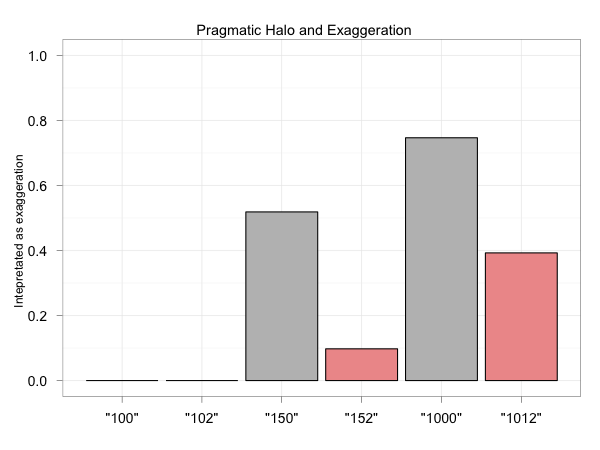
\includegraphics[width=\textwidth]{model_halo_exaggeration.png}
		\caption{Pragmatic Halo and Exaggeration}
	\end{subfigure}
	 \begin{subfigure}[b]{0.33\textwidth}
                \centering
                %\includegraphics[width=\textwidth]{}
		\caption{can fit more plot here}
	\end{subfigure}
	\caption{The graph on the left shows rah rah rah and the one on the right shows roar roar roar}
\end{figure}

\subsection{Hyperbole}

Hyperbole is similar to exaggeration, except that additional information about the \emph{valence} of the meaning is conveyed. Valence is a second dimension of meaning, separate from the number that the speaker wants to convey. If $V$ is the set of possible valences, then the set of possible meanings $M$ is given by:
\begin{equation}
M = [a,...,b] \times V.
\end{equation}

The model of hyperbole is similar to the exaggeration model, except that it needs to be compatible with meanings that consist of number-valence pairs. The dictionary entry $\dictionary_u$ for an utterance $u$ now consists of a Gaussian centered around $u$, as before, as well as a truth function $T_u:V\rightarrow \{0,1\}$ that determines which valences are compatible with $u$. This leads us to modify equation \ref{eq:literallistener} so that the literal listener is now defined by:

\begin{align}\label{eq:valenceliteral}
L_0((k,v) | u, \dictionary) &\propto \dictionary_u(k,v)P(k,v) \\
&=f(k;u,\sigma^2)T_u(v)P(k)P(v),
\end{align}
where $k$ is the number that the speaker wants to communicate, $v$ is the valence, and we assume for simplicity that number and valence are independent under the prior. 

The rest of the model is extended in a similar manner. We note that there are now many more possible dictionaries: each utterance is assigned both a standard deviation and a truth function, and there are $2^{|V|}$ truth functions on valences. 

We will now illustrate this model using the simplest example of hyperbole. We assume that there are two number meanings, \emph{1} and \emph{2}, and two valences, \emph{neutral} and \emph{negative}, so that there are four pairings of numbers and valences. We assume that \emph{1} is more likely than \emph{2}, and \emph{neutral} is more likely than \emph{negative}. There are two utterances, ``one" and ``two." If the speaker wants to communicate \emph{1}-\emph{neutral}, she is likely to succeed by saying ``one" whether its dictionary entries are vague or precise, because it is the most \emph{a priori} probable meaning. This speaker will assign small probability to the utterance ``two." On the other hand, there are two moderately likely meanings that may lead the speaker to say ``two": \emph{2}-\emph{neutral} and \emph{1}-\emph{negative}. It is clear why the speaker would say ``two" to communicate the first meaning. For the second meaning, \emph{1}-\emph{negative}, the speaker may use the utterance ``two" if she believes that the number meaning of this utterance is vague (and therefore compatible with meaning \emph{1}) and that it uniquely picks out the negative valence. Because ``two" may be used to communicate this meaning, it provides evidence to the listener that this meaning was intended. This is the hyperbolic interpretation of the utterance ``two." 

\subsection{The complete model}

Our final model combines the elements of the previous models. It is intended to simultaneously capture three effects: pragmatic halo, the interpretation of extreme utterances as exaggerated, and the interpretation of exaggerated utterances as hyperbolic. This model will allow the costs of utterances to vary, as in the model of pragmatic halo; allow prior probabilities of meanings to vary, as in the model of exaggeration; and introduce valences into the meaning, as in the model of hyperbole. Formally, the model will be identical to the model of hyperbole, except that we allow for utterance costs $c(u) > 0$. 

\section{Behavioral Experiment}

We conducted a behavioral experiment to test whether human interpretations of potentially hyperbolic statements can be explained using the model we proposed. We tested the model on five different scenarios. In each scenario, a speaker makes an utterance that contains a numerical value that conveys information about a particular item or state of the world, for example, the price of a textbook or the temperature outside. Subjects are asked to judge whether the utterance was an exaggeration or a literal statement, as well as what they think the actual state of the world was.
\subsection{Procedures}

We recruited $220$ subjects located in the United States through Amazon Mechanical Turk. $4$ of the subjects were non-native English speakers, and their responses were excluded from the analysis. Each subject read five short scenarios in random order regarding the following five domains: the number of minutes a bus is behind schedule, the price of a college textbook, the cost of a parking ticket, the number of pages in a reading assignment, and the weather temperature (in degrees Fahrenheit). We selected these domains because we believe people have reliable intuitions about the true distributions of such values, and also because people are likely to exaggerate and express an opinion about these issues. 

% How to best present this material?

Each scenario was structured in a similar manner. Below is an example of the textbook scenario:\\\\
\emph{Ann and Bob are friends. They are taking the same class.\\
\textbf{Ann:}  ``How much did the textbook cost?"\\
\textbf{Bob:} ``\{X\} dollars."\\
}
\\After reading the scenario, subjects then answered the following questions:
\emph{
\begin{itemize}
\item[(1)] Was Bob being literal about the temperature, or was he exaggerating? [literal / exaggerating]
\item[(2)] What do you think the temperature actually is? [free response]
\item[(3)] How negative does Bob feel about the temperature?
\item[(4)] What was Bob most likely trying to communicate by saying: ``\{X\} degrees Fahrenheit?" [It is exactly \{X\} degrees Fahrenheit / It is approximately \{X\} degrees Fahrenheit / It is very hot and Bob is not happy about it.
\end{itemize}
}

% A paragraph here explaining why we asked the questions we did and what effects we expect to see (our hypotheses).
Based on our model and theory of the pragmatic interpretation of numbers, we predict that subjects' responses will exhibit the following phenomena:
\begin{itemize}
\item[(1)] Pragmatic halo: round numbers are interpreted less precisely and literally
\item[(2)] Exaggeration: less likely numbers are interpreted as closer to the mean
\item[(3)] Valence: exaggerated utterances are interpreted as having marked meaning and stronger valence
\item[(4)] Interaction of all three elements above, such that it reflects the actual interpretation of how humans communicate with hyperbole.
\end{itemize}
%%%%

\subsection{Results}
\begin{figure}
        \begin{subfigure}[b]{0.5\textwidth}
                \centering
		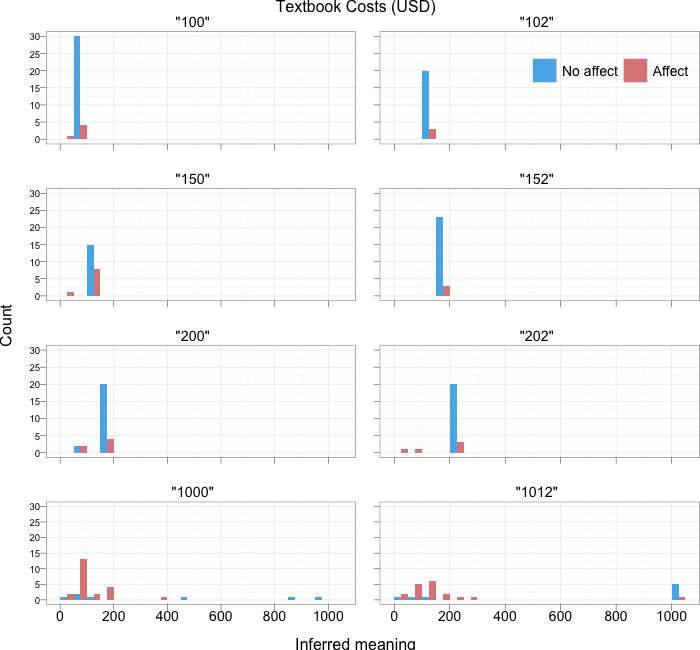
\includegraphics[width=\textwidth]{humans_all_textbook.png}
		\caption{textbooks}
	\end{subfigure}
        \begin{subfigure}[b]{0.5\textwidth}
                \centering
                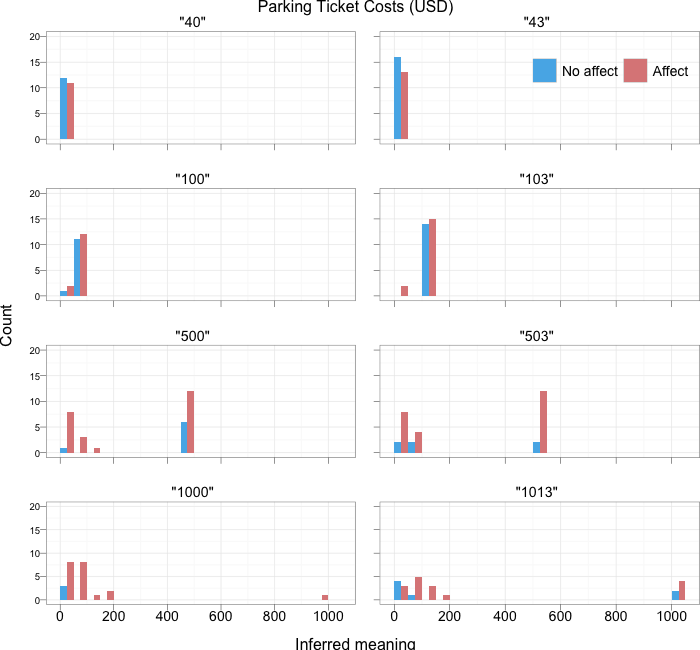
\includegraphics[width=\textwidth]{humans_all_ticket.png}
		\caption{tickets}
	\end{subfigure}
	\begin{subfigure}[b]{0.33\textwidth}
                \centering
                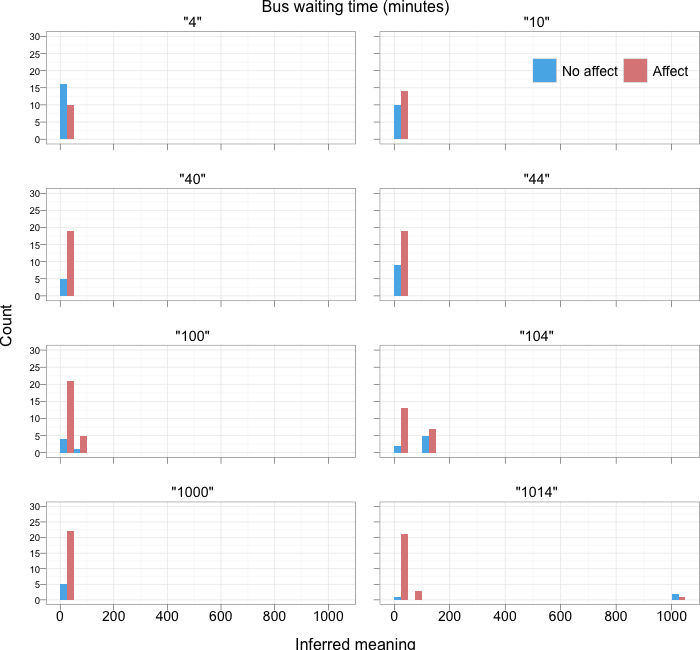
\includegraphics[width=\textwidth]{humans_all_bus.png}
		\caption{bus wait time}
	\end{subfigure}
	\begin{subfigure}[b]{0.33\textwidth}
                \centering
                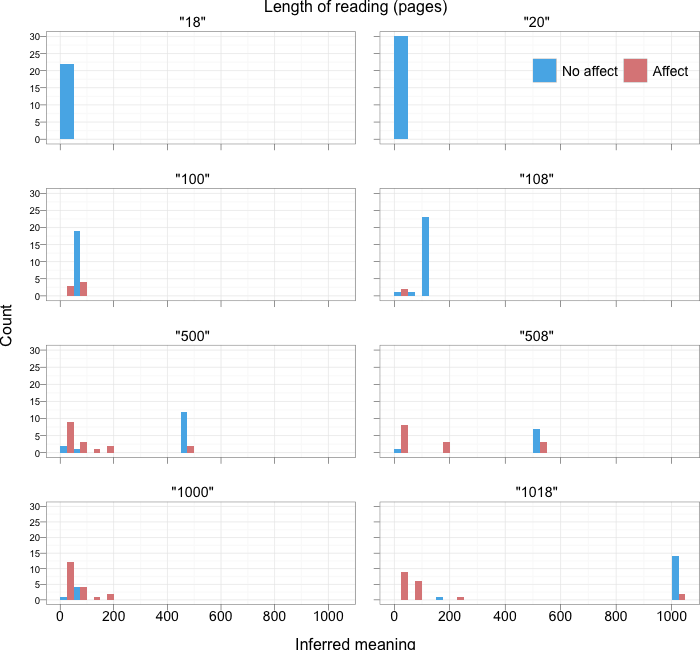
\includegraphics[width=\textwidth]{humans_all_reading.png}
		\caption{reading assignment}
	\end{subfigure}
	\begin{subfigure}[b]{0.33\textwidth}
                \centering
                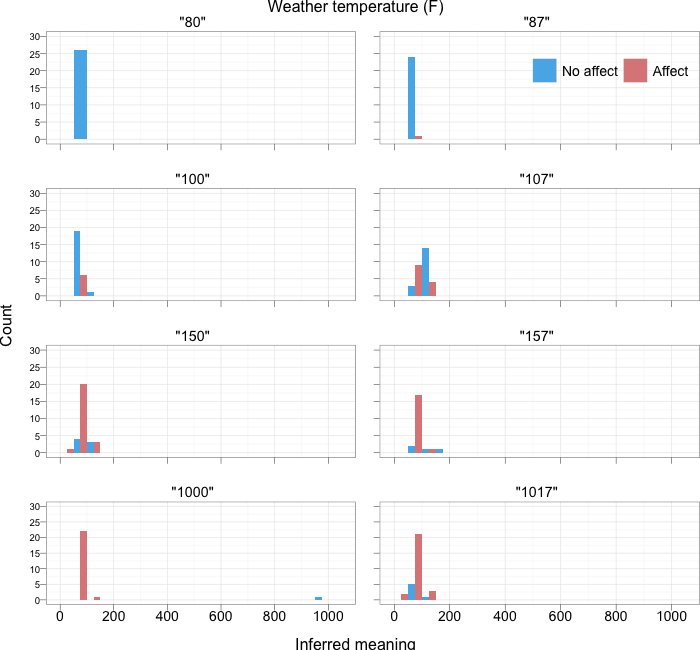
\includegraphics[width=\textwidth]{humans_all_weather.png}
		\caption{weather temperature}
	\end{subfigure}
	\caption{These graphs show the relationship between uttered values and its probability of being perceived to convey affect.}
\end{figure}


% halo and exaggeration

\begin{figure}
        \begin{subfigure}[b]{0.5\textwidth}
                \centering
		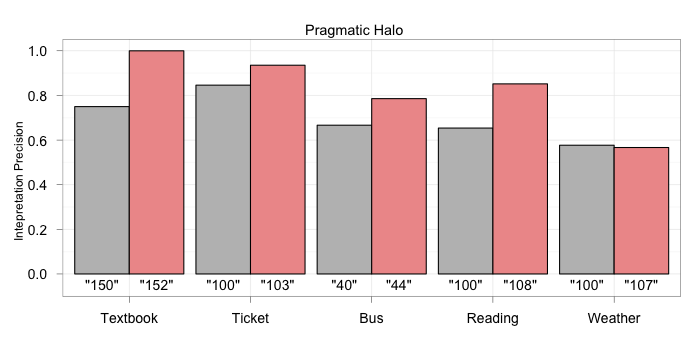
\includegraphics[width=\textwidth]{humans_halo.png}
		\caption{halo effect}
	\end{subfigure}
        \begin{subfigure}[b]{0.5\textwidth}
                \centering
                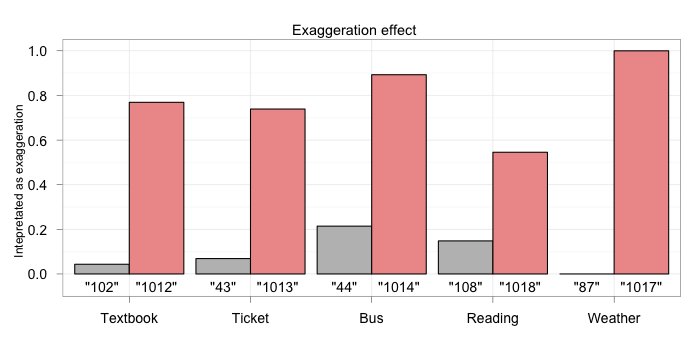
\includegraphics[width=\textwidth]{humans_exagg.png}
		\caption{exaggeration}
	\end{subfigure}
	\caption{The graph on the left shows rah rah rah and the one on the right shows roar roar roar}
\end{figure}

% halo & exaggeration
The results are consistent with our model predictions. The proportion of subjects who interpreted an utterance as hyperbolic varies as a function of the distance between uttered and expected values as well as the ``roundness" of the uttered value. 
As shown in Figure 1, subjects' responses demonstrates a pragmatic halo effect, in which precise numbers are interpreted more literally than round numbers. Subjects are also more likely to judge an utterance as exaggeration when the literal meaning of the numeric value becomes less likely in a particular domain. For instant, when prompting subjects to a temperature of 107 degrees Fahrenheit, they judged it as exaggeration because it is unlikely that the weather gets that high in the United States, from which these subjects were recruited.

% exaggeration and affect
We then analyzed how perception of hyperbolic intent and distance between the uttered price and expected price interacted to form subjects' inferences of the actual price. Figure 3(a) shows the average of subjects' inferred prices given different uttered prices and whether or not they interpreted the utterance as a hyperbole. When subjects perceived a hyperbolic intent, they inferred that the actual price was less than the uttered price and closer to the expected (mean) price. When the uttered price became very unlikely, for example when the uttered price was \texttt{1000}, subjects inferred that the actual price is very close to the mean. When subjects did not perceive a hyperbolic intent, however, they inferred that the actual price was close to the uttered price. Figure 3(b) shows the relationship between exaggeration and valence effects. Utterances that were interpreted as exaggeration conveyed significantly higher negative affect than utterances that were interpreted literally. 

% everything

\section{Comparison and Discussion}
Our model captures some important intuitions regarding the numerical values and statistical properties of the uttered price. Here we compare our model results and behavioral data on two aspects: (1) Probability of interpreting the utterance as hyperbolic (2) Most likely inferred price given that the utterance is interpreted as hyperbolic or literal.


As shown in Figure 7, the probability that the model interprets the utterance as hyperbolic roughly matches that of the behavioral data, at least in the general trend. It appears that humans are less affected by the actual uttered price and are similarly likely to interpret the utterance as hyperbole when $U = 200$ and when $U = 1000$.


\begin{figure}
        \begin{subfigure}[b]{0.5\textwidth}
                \centering
		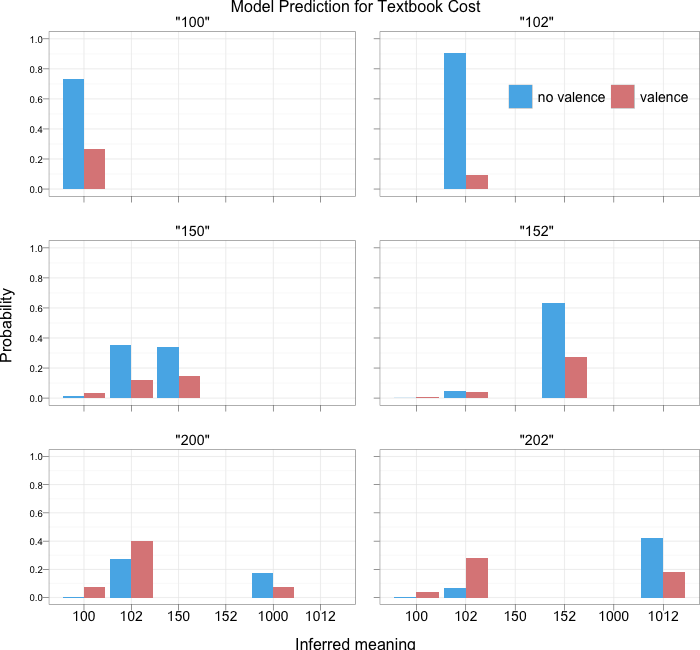
\includegraphics[width=\textwidth]{model_all_textbook.png}
		\caption{model all textbook}
	\end{subfigure}
        \begin{subfigure}[b]{0.5\textwidth}
                \centering
                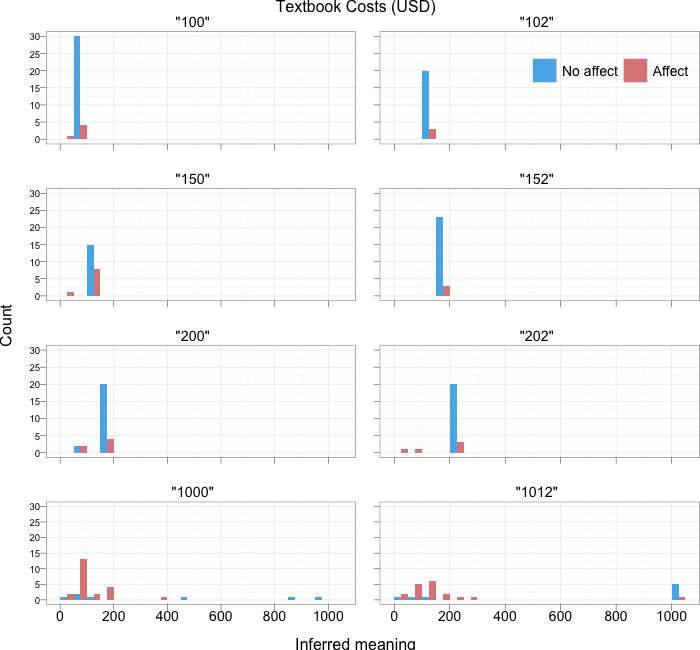
\includegraphics[width=\textwidth]{humans_all_textbook.png}
		\caption{humans all textbook}
	\end{subfigure}
	\caption{The graph on the left shows rah rah rah and the one on the right shows roar roar roar}
\end{figure}


Figure 8 shows the model and humans' inferred prices when there is no perceived hyperbolic intent. Since the model and participants alike interpret the utterance literally and believe that $A = U$, the model predictions almost perfectly match the human responses. Interestingly, the model and humans also infer a similar price when $U = 1000$. Our model infers a value of close to $100$ even when it detects no hyperbolic intent, because the prior probability $P(A = 1000, O = \text{no opinion})$ is extremely low. We are not sure why humans also have this interpretation, although it would  be interesting to examine and verify with further data.


Figure 9 shows the model and humans' inferred prices when listener interprets utterance as hyperbolic. We see that there is a fairly good fit when the uttered prices are close to the mean. However, while the model prediction drops close to the mean when $U > 200$, humans' inferred prices follow the uttered prices fairly closely until $U = 1000$. However, since we did not ask humans to make these inferences when $ 250 < U < 1000$, it is unclear if humans' inferred price will also fall back to the mean steadily after a certain threshold price. In general, it appears that human subjects are more willing to believe the speaker. It may also be that Stanford students are more cynical about textbook prices and readily believe in textbooks that cost $250$ dollars.


\section{Future Directions \& Conclusion}
Although our model is able to capture the fundamentals of hyperbolic interpretation in this particularly simplistic scenario, more work is needed to extend the model to more complicated settings and generic domains. We would also like to focus on improving the recursive model of a speaker and a listener to better represent the listener's internal model for the speaker, and vice versa. Lastly, our future work will attempt at modeling a speaker's opinion as part of her communicative goals in a conversation, and how a listener can infer the intended meaning.

\subsubsection*{References}

\small{
[1] Alexander, J.A. \& Mozer, M.C. (1995) Template-based algorithms
for connectionist rule extraction. In G. Tesauro, D. S. Touretzky
and T.K. Leen (eds.), {\it Advances in Neural Information Processing
Systems 7}, pp. 609-616. Cambridge, MA: MIT Press.

[2] Bower, J.M. \& Beeman, D. (1995) {\it The Book of GENESIS: Exploring
Realistic Neural Models with the GEneral NEural SImulation System.}
New York: TELOS/Springer-Verlag.

[3] Hasselmo, M.E., Schnell, E. \& Barkai, E. (1995) Dynamics of learning
and recall at excitatory recurrent synapses and cholinergic modulation
in rat hippocampal region CA3. {\it Journal of Neuroscience}
{\bf 15}(7):5249-5262.
}

\bibliographystyle{apacite}

\setlength{\bibleftmargin}{.125in}
\setlength{\bibindent}{-\bibleftmargin}

\bibliography{nips_hyperbole}


\end{document}
